% !TeX spellcheck = it_IT
% !TEX encoding = utf8
% !TEX root = main.tex

\chapter{Gauss - Il principe dei Matematici}
\begin{minipage}{1.46\linewidth}
	\begin{flushright}
		\emph{La matematica è la regina delle scienze \\ e la teoria dei numeri è la regina della matematica.}\\
		\vspace{0.5cm}
		\bfseries{Carl Friedrich Gauss} \\
		\textnormal{(Braunschweig, mercoledì 30 aprile 1777-\\Gottinga, Venerdì 23 febbraio 1855)}.
	\end{flushright}
\end{minipage}

Carl Friedrich Gauss è stato probabilmente il più poliedrico scienziato di tutti i tempi ed è stato il penultimo uomo a "sapere tutto" (è stato superato solo parecchio tempo dopo da un certo Poincaré). Durante la sua lunghissima e vastissima produzione scientifica, è stato matematico, fisico e astronomo.

Ha dato contributi fondamentali in tutte le branche della matematica e della fisica allora conosciute: dall'analisi matematica (sia reale che complessa vedi articolo sui numeri complessi) alla teoria dei numeri, statistica, calcolo numerico, geometria differenziale, geodesia, geofisica, al magnetismo e elettrostatica fino all'astronomia e all'ottica.

\marginpar{
	\captionsetup{type=figure}
	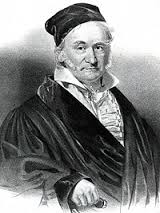
\includegraphics[width=\marginparwidth]{gauss.jpeg}
	\caption[Ritratto di Gauss]{Ritratto di Gauss}
	\label{fig:gauss}
}


Viene ricordato come Universalista, dal momento che eccelse in tutti i campi della disciplina nota ai suoi giorni.

\section{L'enfant prodige}

La storiografia insegna che fin dai primi anni di vita è stato considerato come un bambino prodigio. Molti aneddoti sono raccontati sulla sua infanzia, certi più famosi di altri, certi più accreditati di altri.

In particolare due sono particolarmente conosciuti:
\begin{itemize}
	\item Si narra che all'età di tre anni abbia corretto dei calcoli nelle finanze del padre; già dopo pochi mesi di vita, Gauss era in grado di fare operazioni algebriche, leggere e addirittura scrivere qualcosa.
	\item Un altro aneddoto racconta di come il suo il suo pigro insegnante, J.G. B\"{u}ttner, per tenere occupati i suoi allievi, ordinò loro di fare la somma dei numeri da 1 a 100. A quel tempo il giovane Gauss aveva solo 9 anni ma ugualmente dopo pochi minuti riuscì a consegnare la somma corretta: 5050.
\end{itemize}
Molte ipotesi sono state avanzate su quale metodo Gauss abbia usato: l'ipotesi più accreditata è che Carl si sia accorto che i numeri che differiscono della stessa distanza dagli estremi della serie danno sempre la stessa somma. Probabilmente mise in una riga i numeri da 1 a 100 e in una riga sotto i numeri da 100 a 1, e vide che ogni colonna dava come somma 101:

\[\begin{tabular}{cccccc}
$1$  &  $2$  &  $\dots $ & $99$  &  $100$ & $ + $\\
$100$  &  $99$  &  $\dots $ & $2$  &  $1$ & $ = $ \\ \hline
$101$  &  $101$  &  $\dots $ & $101$  &  $101$ & $  $\\
\end{tabular}\]

non restava dunque che fare il semplice calcolo $ \frac{100 \times 101}{2} $, ottenendo il risultato 5050 appunto. Aveva appena scoperto a 9 anni il risultato di quello che adesso noi chiameremo \emph{somma aritmetica}, o in simboli

\[\sum_{n=1}^{N} n  = \frac{N\times(N+1)}{2}  \] 

B\"uttner deve arrendersi davanti all'evidenza e dopo poco tempo supplicherà il il Duca di Brunswick di finanziare il giovane prodigio per potergli permettere di proseguire gli studi all'Università di Braunschweig prima (la più antica di Germania) e di Gottinga poi, dove trascorse gran parte del resto della sua esistenza.

\section{L'annus aureus}

Giunto all'Università Gauss ottenne una serie di notevoli risultati. Finalmente il suo genio poteva esprimersi al meglio e soprattutto poteva essere supportato e indirizzato da professori del suo livello, perlomeno fintanto che non vennero surclassati. In particolare il 1796 viene ricordato come l'anno d'oro. 
\marginpar{
	\captionsetup{type=figure}
	
\includegraphics[width=\marginparwidth]{firmaGauss}
	\caption{Firma di Gauss; si può notare come sia riuscito a conciliare nel suo nome il simbolo di integrale, la lettera greca $ \pi $ e il numero di Nepero $ e $}
	\label{fig:firmaGauss}
}
Tra le maggiori scoperte possiamo citare:
\begin{itemize}
	\item riuscì a dimostrare che un poligono regolare con un numero di lati che è un primo di Fermat è costruibile con riga e compasso. Questa fu una grande scoperta in un importante campo della matematica; la costruzione dei poligoni aveva occupato i matematici fin dall'epoca degli antichi greci, e la scoperta dette modo a Gauss di scegliere di intraprendere la carriera di matematico anziché di filologo.
	\item riuscì a costruire un eptadecagono;
	\item inventò l'aritmetica modulare, importantissimo strumento della teoria dei numeri che, solo per inciso, è la teoria dei numeri che tiene al sicuro i vostri e i miei soldi in banca;
	\item congetturò per primo la validità del teorema dei numeri primi, dando un'idea chiara di come i numeri primi siano distribuiti fra gli interi, cioè che se ne trovano sempre più di rado mano a mano che ci spostiamo verso l'infinito in un'ipotetica linea dei numeri, ma la loro distribuzione segue un andamento logaritmico;
	\item scoprì che tutti i numeri naturali sono rappresentabili al più come somma di tre numeri triangolari (Un numero intero positivo si dice triangolare se è uguale alla somma di una sequenza di numeri naturali consecutivi a partire da 1).
\end{itemize}

Aveva appena 19 anni. Per darvi l'idea, un ragazzo normale che studia matematica come il sottoscritto, non ha i mezzi per comprendere nemmeno un risultato. E pensatevi che molti dei suoi risultati sono stati pubblicati postumi o comunque dopo molti anni: voleva che fossero perfetti e riteneva molte delle dimostrazioni "non eleganti ".

A 22 anni completa il dottorato a Gottinga: nella sua tesi di dottorato viene riportata una nuova dimostrazione del teorema per il quale ogni funzione algebrica integrale di una variabile può essere risolta in fattori di primo o secondo grado. Aveva appena dimostrato il teorema fondamentale dell'algebra. Era entrato nella storia.

Sfortunatamente per lui, era troppo avanti rispetto ai suoi contemporanei; la sua commissione giudicatrice non aveva i mezzi necessari per capire la sua dimostrazione e verrà completamente appresa grazie al lavoro del geometra (in senso matematico, sia chiaro  ) francese Jordan e alla completa definizione dei numeri complessi.

Per non farsi mancare nulla, prima della sua morte pubblicò altre 4 dimostrazioni di questo teorema.

\section{La maturità}

Nel 1801, all'età di 24 anni, presenta il suo lavoro "\emph{Disquisitiones Arithmeticae}" che si rileva subito
come un dei contributi più importanti alla teoria dei numeri e una pietra miliare nel campo della matematica, al pari dei "\emph{Principia Mathematica}" di Newton.

In questo lavoro Gauss introduce ancora alcune nozioni basilari: i già citati numeri complessi, o immaginari- anche se di immaginario hanno poco- e la teoria delle congruenze. Il testo contiene anche una dimostrazione della legge di reciprocità quadratica (riguarda la risolubilità relativa in aritmetica modulare di due equazioni quadratiche correlate, dando le condizioni per cui entrambe, nessuna o una sola di esse hanno soluzione); un risultato che Gauss giudicava così importante che ne diede varie dimostrazioni durante la sua vita.

\subsection{Astronomia}
Per non farsi mancare nulla, si appassionò di li a poco tempo di astronomia: attraverso l'elaborazione di un nuovo metodo per la definizione delle orbite dei corpi celesti, infatti, riesce a calcolare la posizione dell'asteroide Cerere.

Il problema era stato lanciato da un astronomo italiano che dopo essere riuscito a tracciare la posizione dell'asteroide per un paio di mesi, ne aveva perso le tracce a causa del bagliore del sole. Dopo tre mesi di duro lavoro predisse la posizione di Cerere nel dicembre 1801 - appena un anno dopo il suo primo avvistamento - con un errore di appena mezzo grado.

Introdusse la costante gravitazionale di Gauss, e sviluppò il cosiddetto metodo dei minimi quadrati, una procedura usatissima ancora oggi per minimizzare l'impatto degli errori di misurazione. Questo risultato gli vale una posizione all'Osservatorio di Goettingen, di cui nel tempo ne diventerà direttore. Lo rimarrà fino alla morte.

\subsection{Probabilità}

Parallelamente ai lavori sull'astronomia, sviluppò una serie di fondamentali strumenti sull'analisi di dati e sulla distribuzione asintotica degli errori di misurazione. Stiamo parlando del teorema fondante della statistica e dell'econometria: il Teorema di Gauss-Markov.

\subsection{Geodetiche e Geometrie non euclidee}

Incaricato dal duca di Hannover nel 1821 a effettuare degli studi sui suoi possedimenti, Gauss diventa il principale studioso della cosiddetta geometria non-euclidea (purtroppo non mi posso dilungare troppo su questo punto, altrimenti un articolo non basterebbe per sviluppare solo questo paragrafo). Durante questo periodo sviluppa la teoria delle superfici e scopre il \emph{Teorema Egregium}(con tutto il rispetto per gli altri teoremi).

Parallelamente sviluppa anche quella che poi sarebbe stata chiamata "geometria sferica" negando il $ V $ postulato della geometria di Euclide. L'argomento però era scottante e Gauss decise di non pubblicare il risultato. Svariati anni dopo, il figlio di un suo intimo amico, dicasi Janos Bolyai, gli invia un lavoro rivoluzionario nel quale si sviluppano delle considerazioni sulla negazione del $ V $ postulato.

Gauss gli rivela privatamente che lo aveva anticipato di 30 anni. Questo amareggiò molto Janos, che mise fine ai rapporti con Gauss pensando che egli stesse rubando l'idea. Oggi la precedenza di Gauss è appurata ma quest'ultimo si rifiutò di pubblicare il lavoro per il timore della controversia.

\subsection{Elettromagnetismo}

Intorno al 1830, invece, si interessa di fisica e in particolare dei fenomeni che regolano l'elettromagnetismo. Inizia la collaborazione con il fisico Weber. Trova quella che sarà poi definita "legge di Gauss" o "Teorema del flusso" ossia la regola che sta alla base del comportamento delle particelle cariche statiche svelando il segreto che sta alla base della loro interazione: la distanza, in particolare il reciproco della distanza al quadrato.

La legge scopre insomma che tra due cariche elettriche ferme agisce una forza che dipende dalle cariche e dalla distanza a cui si trovano.

\subsection{Curiosità}

Curioso segnalare che il matematico ebbe l'idea di applicare il suo ingegno anche all'economia, questa volta non per soli e nobili fini scientifici ma anche per giustificati fini...personali. Infatti, si dedicò anche ad uno studio accurato dei mercati finanziari fino a guadagnare una fortuna personale considerevole.
\section{Morte e eredità}

Muore a Gottinga il 23 febbraio del 1855. Il suo genio era ormai leggenda.

\smallskip

Molte persone lo consideravano schivo e riservato. Ebbe due mogli ed entrambe morirono giovani. Ebbe 6 figli ed ebbe un rapporto travagliato con quasi tutti. Di tutti i figli di Gauss, si diceva che fosse Wilhelmina ad aver ereditato tratti del talento del padre, ma sfortunatamente morì giovane.

Sebbene avesse avuto alcuni studenti, Gauss era noto per detestare l'insegnamento, e prese parte ad un'unica conferenza scientifica, a Berlino nel 1828. Rare erano le collaborazioni con altri matematici, che lo consideravano solitario e austero. Tuttavia molti dei suoi studenti divennero importanti matematici:
\begin{itemize}
	\item Richard Dedekind, che diede fondamentali contributi alla logica e alla teoria dei numeri;
	\item Bernhard Riemann, che sviluppò sulle orme del maestro gli studi sulle geometrie non euclidee e sulle metriche di cui Einstein non poté fare a meno per la sua teoria della gravitazione;
	\item Friedrich Bessel, matematico, geometra e astronomo.
\end{itemize}
Prima che morisse, Sophie Germain (la seconda più grande matematica di tutti i tempi dopo Emmy Noether) fu raccomandata da Gauss affinché ricevesse anche lei la laurea honoris causa.

\bigskip

Questo è il mio primo articolo; se ti è piaciuto, se non ti è piaciuto per niente, se hai qualche annotazione, se mi sono dimenticato qualcosa che pensi sia rilevante (come se ce ne fossero poche :) ) o anche se solo vuoi confrontarti su qualche argomento che ho citato, ti prego di dirmelo; ogni commento è ben accetto ;)

Ho voluto iniziare la mia lista di articoli proprio con Gauss perché ritengo che sia stato il più grande di tutti i tempi e da quando ho iniziato a studiare, non ho ancora trovato una materia in cui prima o poi non si faccia uso di uno dei teoremi di Gauss. Era in anticipo sui suoi contemporanei di 30 o addirittura 50 anni. Senza di lui, probabilmente molti problemi avrebbero ancora il punto interrogativo al posto della soluzione.

\bibliography{bibliography}
\bibliographystyle{plain}


%\bibliography{bibliography}
%\bibliographystyle{plain}
